\documentclass{article}

%%%% 
%%%% try also class: {IEEEtran}
%%%%

\usepackage{graphicx}
\input list
%%%\lstset{language=C,style=demostyle}

\begin{document}
\title{Homework 4:Compile Runtime Assignment}
\author{Justin Campbell \\
UT eID: jsc4348 \\
SDS 335 \\
Dr. Eijkhout}
\date{September 29th 2021}
\maketitle

%% The control structure "\section" can 
%% be used to create paragraphs in latex

\section{First Iteration of Compile Exercise: No Transformations}

In this section, images of the source file, "rotate.c" without any transformations, and the compiler runtimes of the program as they appear in the terminal using compilers, "gcc - O0", "gcc -01", "gcc -02", and "gcc -03" will be provided. This serves as a baseline with which to compare the compiler runtimes for each successive code transformation.

Provided below is a screenshot of the program, "rotate.c" in the first iteration (with no transformations):

%% Insertion of program screenshot using "\includegraphics" command

\begin{figure}[ht]
    \centering
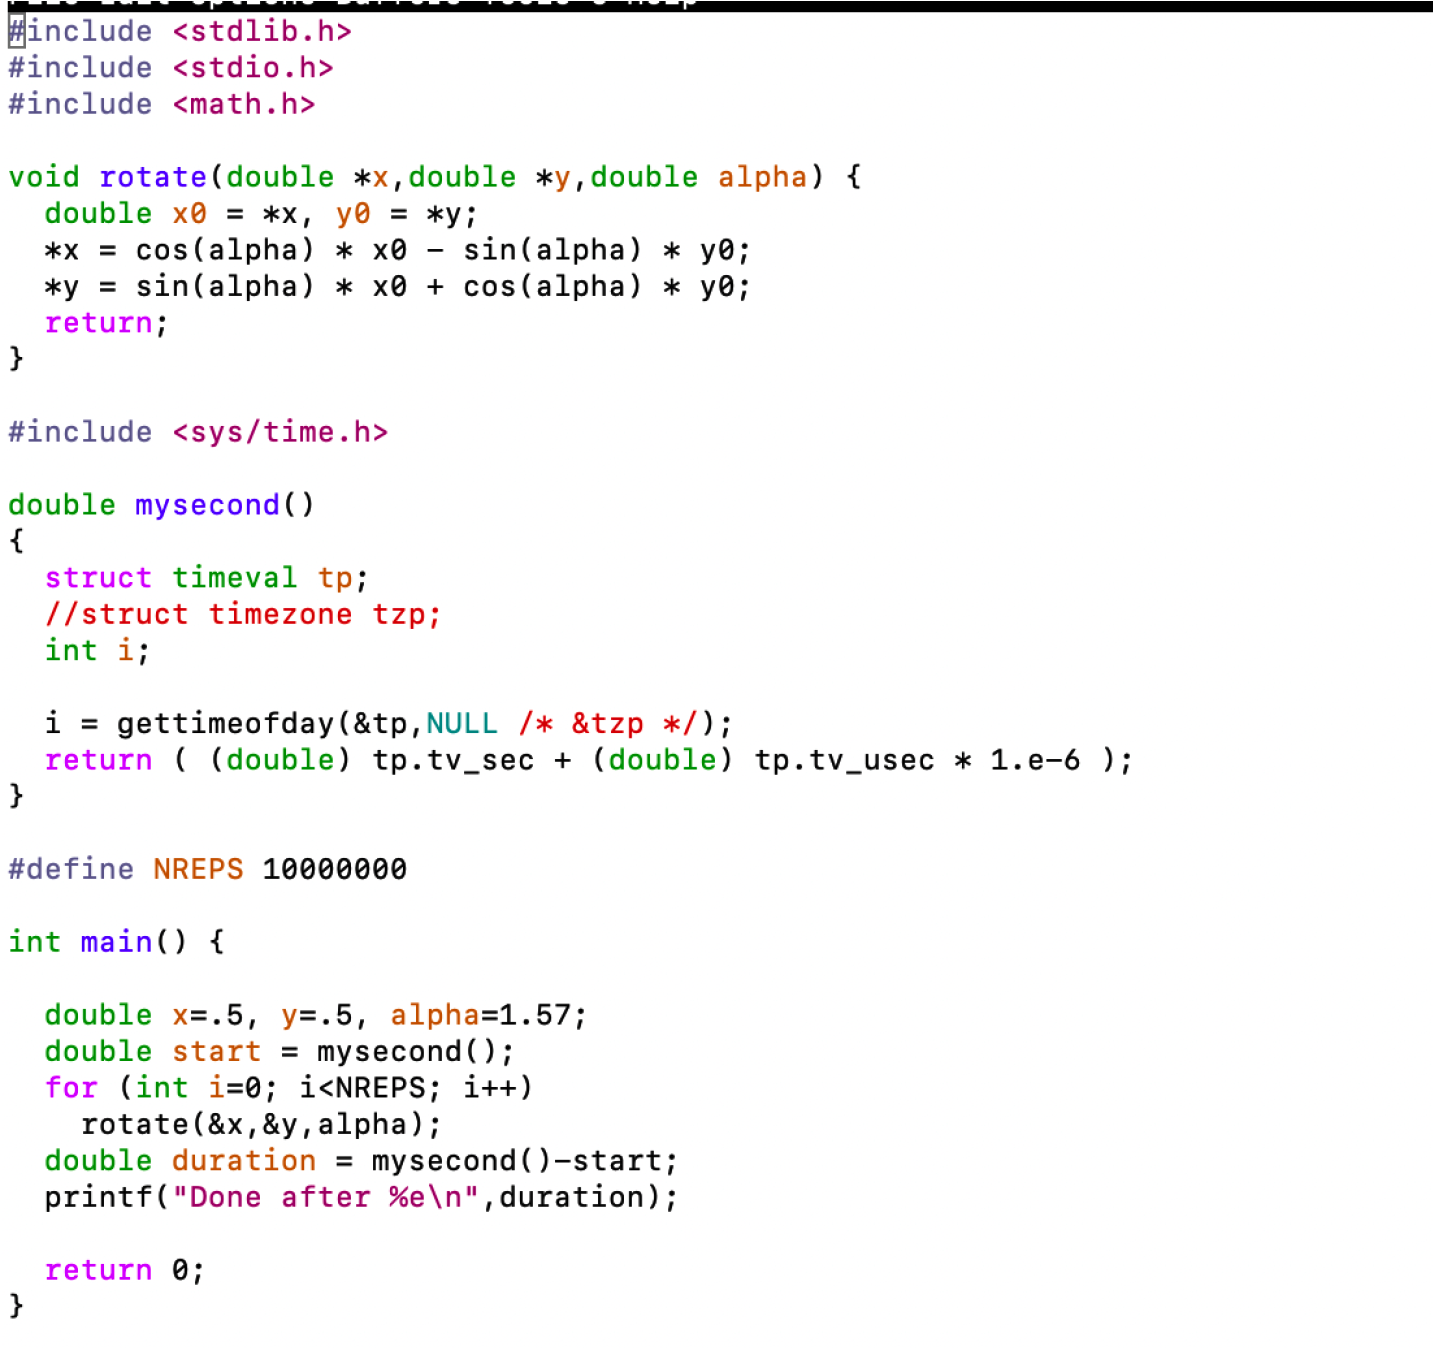
\includegraphics[scale=0.20]{graphics_hw4/rotate_c_first_iteration.png}
    \caption{Screenshot of Program "rotate.c" for First Iteration}
    \label{fig:my_label}
\end{figure}
\pagebreak

%% Insertion of screenshot of compiler runtimes for first iteration of program

\begin{figure}[!h]
    \centering
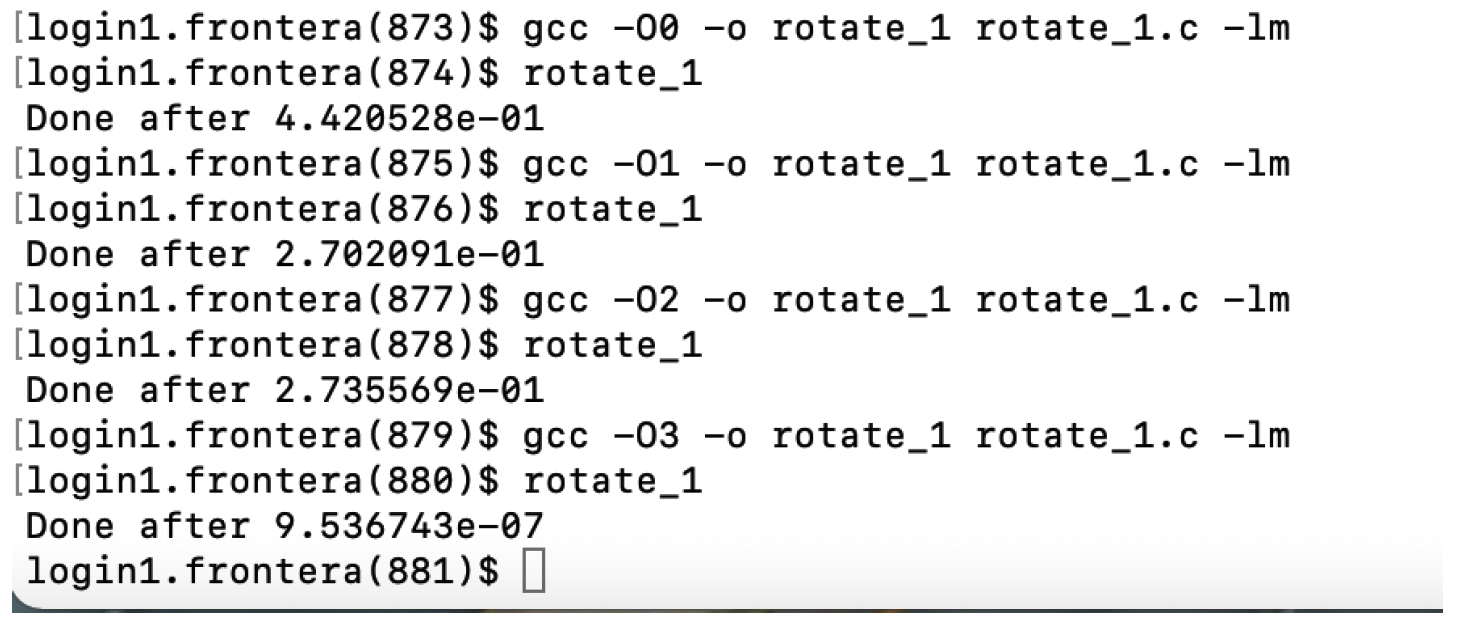
\includegraphics[scale=0.20]{graphics_hw4/compilation_runtimes_first_iteration.png}
    \caption{Screenshot of Compiler Runtimes for First Iteration}
    \label{fig:my_label}
\end{figure}
\pagebreak

%% Summarize observations of runtimes for each of the "gcc" compilers for the first program iteration

Observations:
\begin{enumerate}
    \label{sec:math}
    \item The screenshot presented above provides the compilation commands and associated runtimes for the program, "rotate.c" in decreasing order of runtime (increasing effiency) under the different "gcc" compilers.
    \item We can see that the "gcc-03" compiler improves the performance by a magnitude of $10^{6}$ relative to the "gcc-00" compiler, namely, an improvement from $4.42*10^{-1}$ to $9.54*10^{-7}$
    
\end{enumerate}
\pagebreak

%% Use "\section" command to create a new section to summarize results for second iteration of exercise:

\section{Second Iteration of Compile Exercise: Transformations Applied to Trigonometric Functions}

In this section, images of the source file, "rotate.c" with its first set of transformations, and the compiler runtimes of the program as they appear in the terminal using compilers, "gcc - O0", "gcc -01", "gcc -02", and "gcc -03" will be provided. In particular, variables "$cos\_alpha$" and $"sin\_alpha"$ were defined in the "$rotate()$" function definition as a substitute for explicit function calls for "sin" and "cos" in the assignment for "*x" and "*y" as was provided in the original iteration of the source file. This is determined to be good programming practice, and will generally improve the performance of code. The results from this first set of transformations will be used to compare the runtime efficiencies of the first and second iterations of the program.

Provided below is a screenshot of the program, "rotate.c" in the second iteration (with its first set of transformations):

%% Insertion of program screenshot for second iteration using "\includegraphics" command

\begin{figure}[ht]
    \centering
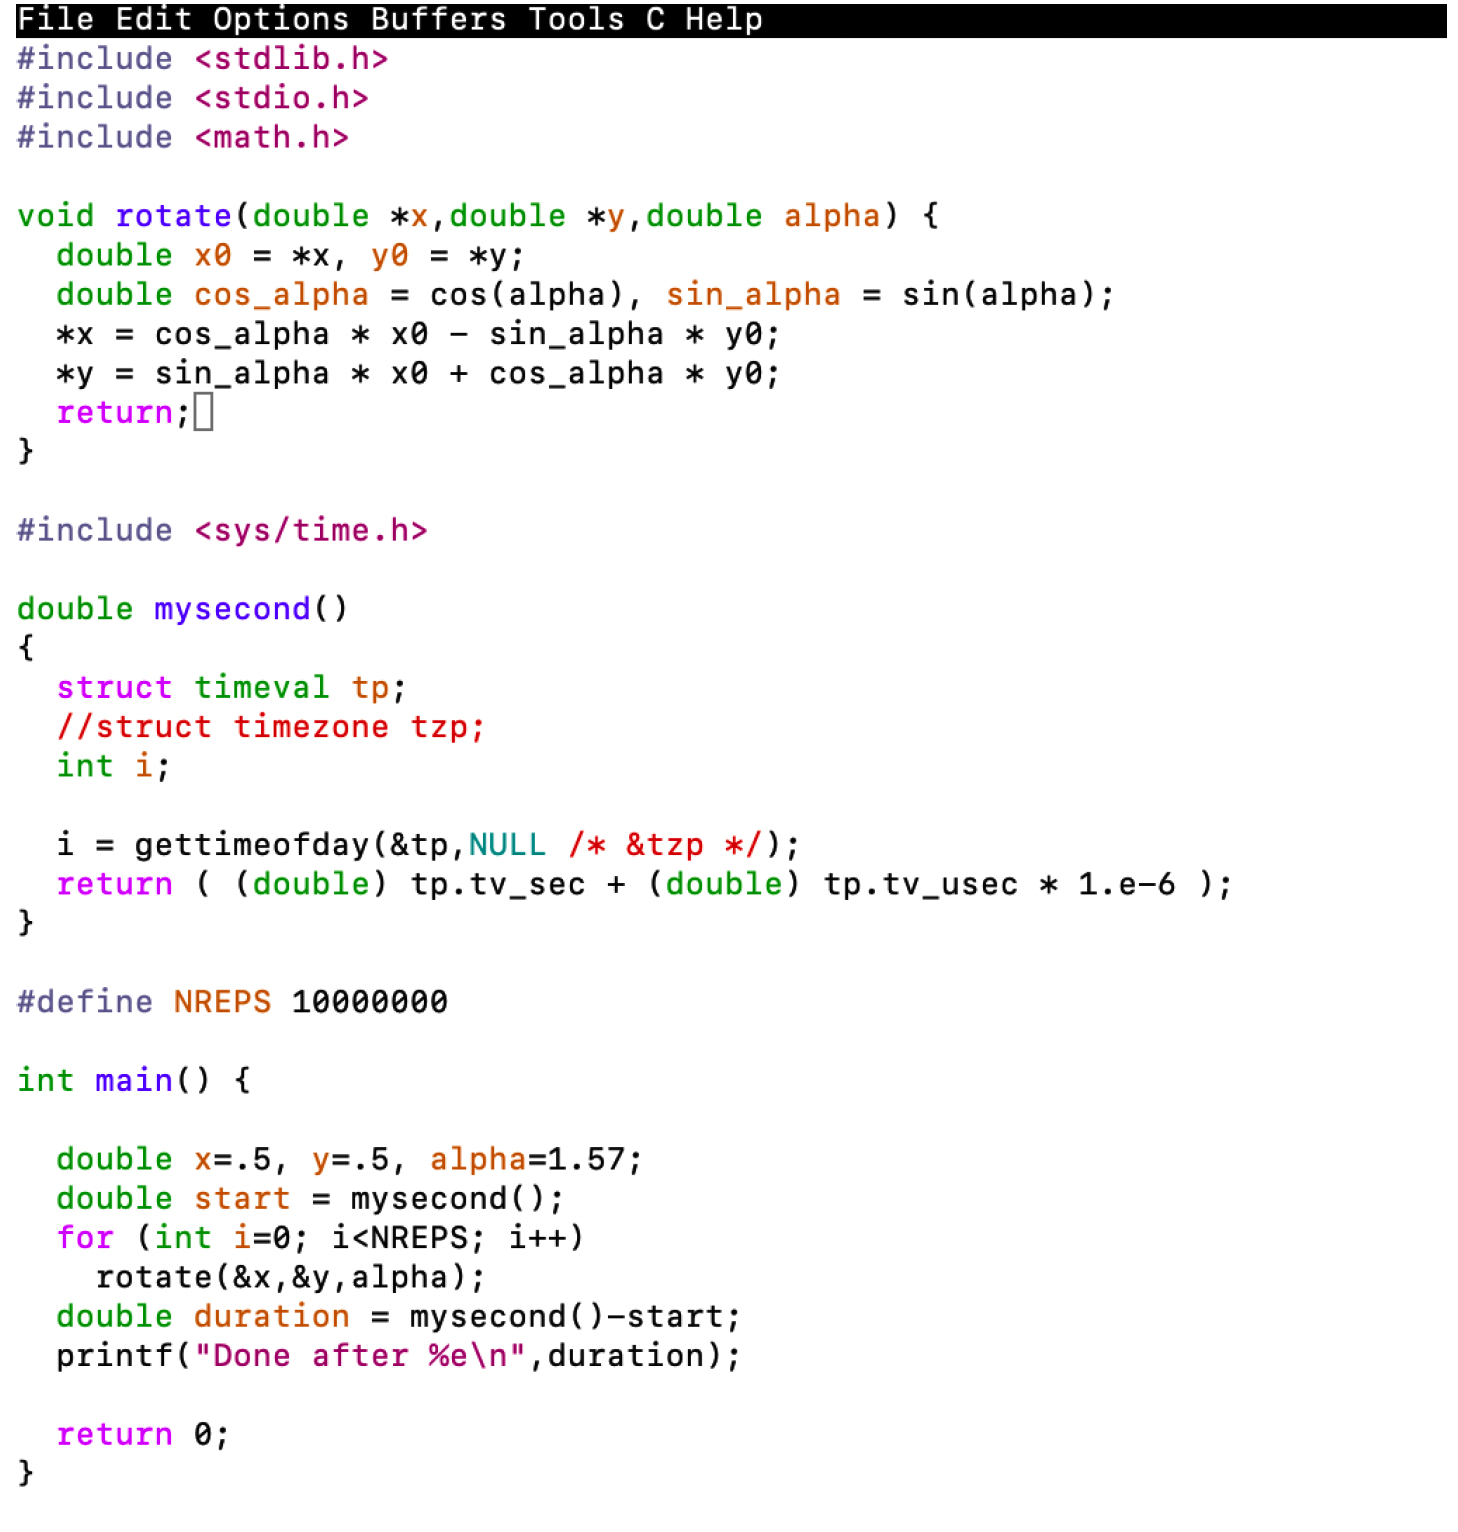
\includegraphics[scale=0.20]{graphics_hw4/rotate_c_second_iteration.png}
    \caption{Screenshot of Program "rotate.c" for Second Iteration}
    \label{fig:my_label}
\end{figure}
\pagebreak


%% Insertion of screenshot of compiler runtimes for second iteration of program

\begin{figure}[!h]
    \centering
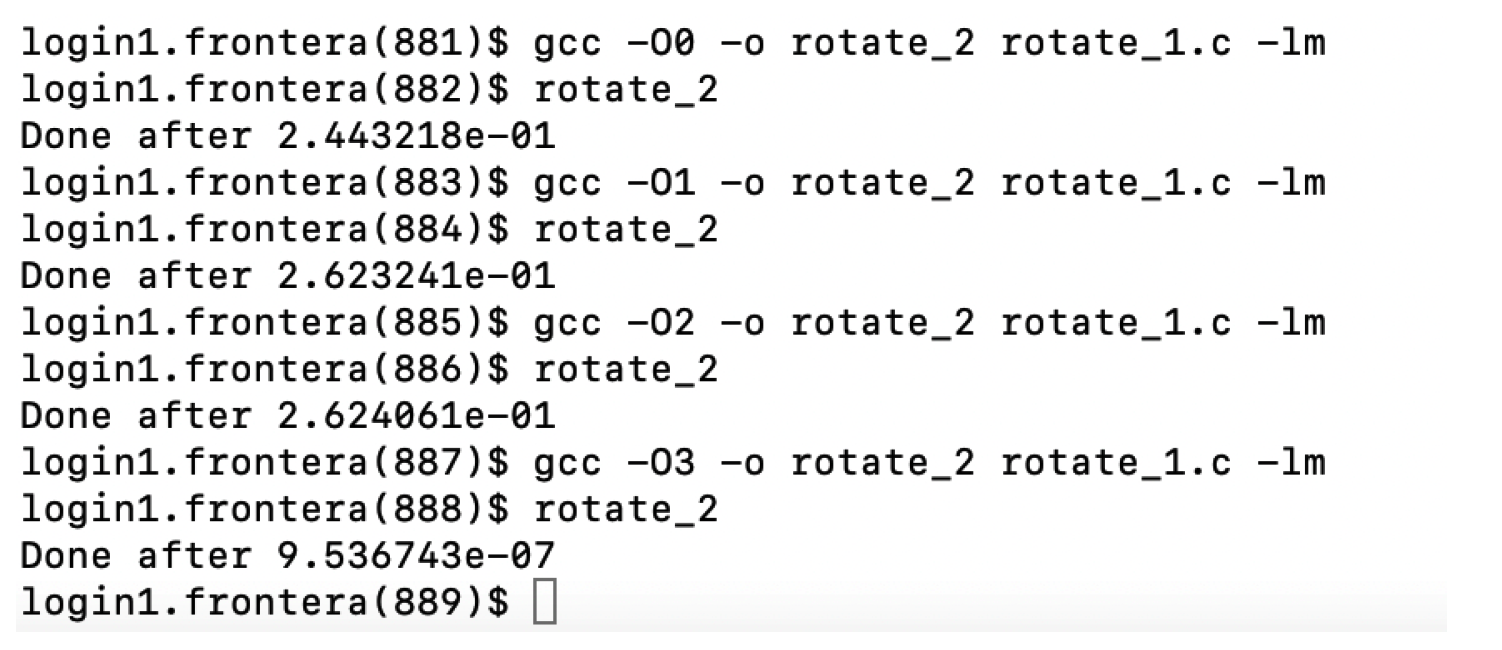
\includegraphics[scale=0.20]{graphics_hw4/compilation_runtimes_second_iteration.png}
    \caption{Screenshot of Compiler Runtimes for Second Iteration}
    \label{fig:my_label}
\end{figure}
\pagebreak

%% Summarize observations of runtimes for each of the "gcc" compilers for the second program iteration

Observations:
\begin{enumerate}
    \label{sec:math}
    \item The screenshot presented above provides the compilation commands and associated runtimes for the program, "rotate.c" in decreasing order of runtime (increasing effiency) after the aforementioned changes to the computations of "*x" and "*y" were applied. 
    \item We can see that the "gcc -03" compiler again improves the performance by a magnitude of $10^{6}$ relative to the "gcc -00" compiler, namely, an improvement from $2.44 * 10^{-1}$ to $9.54 * 10^{-7}$. 
    \item Overall, the performance improvement for the runtime for each compiler is comparable to that of the runtime of the associated compiler for the first iteration of the program. Put differently, this transformation marginally improved the runtime for each compiler and the differences in runtime across the compilers has a similar pattern. 

\end{enumerate}
\pagebreak

%% Use "\section" command to create a new section to summarize results for third iteration of exercise:

\section{Third Iteration of Compile Exercise: Transformations Applied to "printf()" Function Call}

In this section, images of the source file, "rotate.c" with its second set of transformations, and the compiler runtimes of the program as they appear in the terminal using compilers, "gcc - O0", "gcc -01", "gcc -02", and "gcc -03" will be provided. The second set of transformations involved removing the variable declaration "double duration = mysecond() - start", and replacing the argument "duration" with "mysecond() - start" in the "printf()" function call. The results from these transformations will be used to compare the runtime efficiencies of the second and third iterations of the program.

Provided below is a screenshot of the program, "rotate.c" in the third iteration (with its second set of transformations):

%% Insertion of program screenshot for third iteration using "\includegraphics" command

\begin{figure}[ht]
    \centering
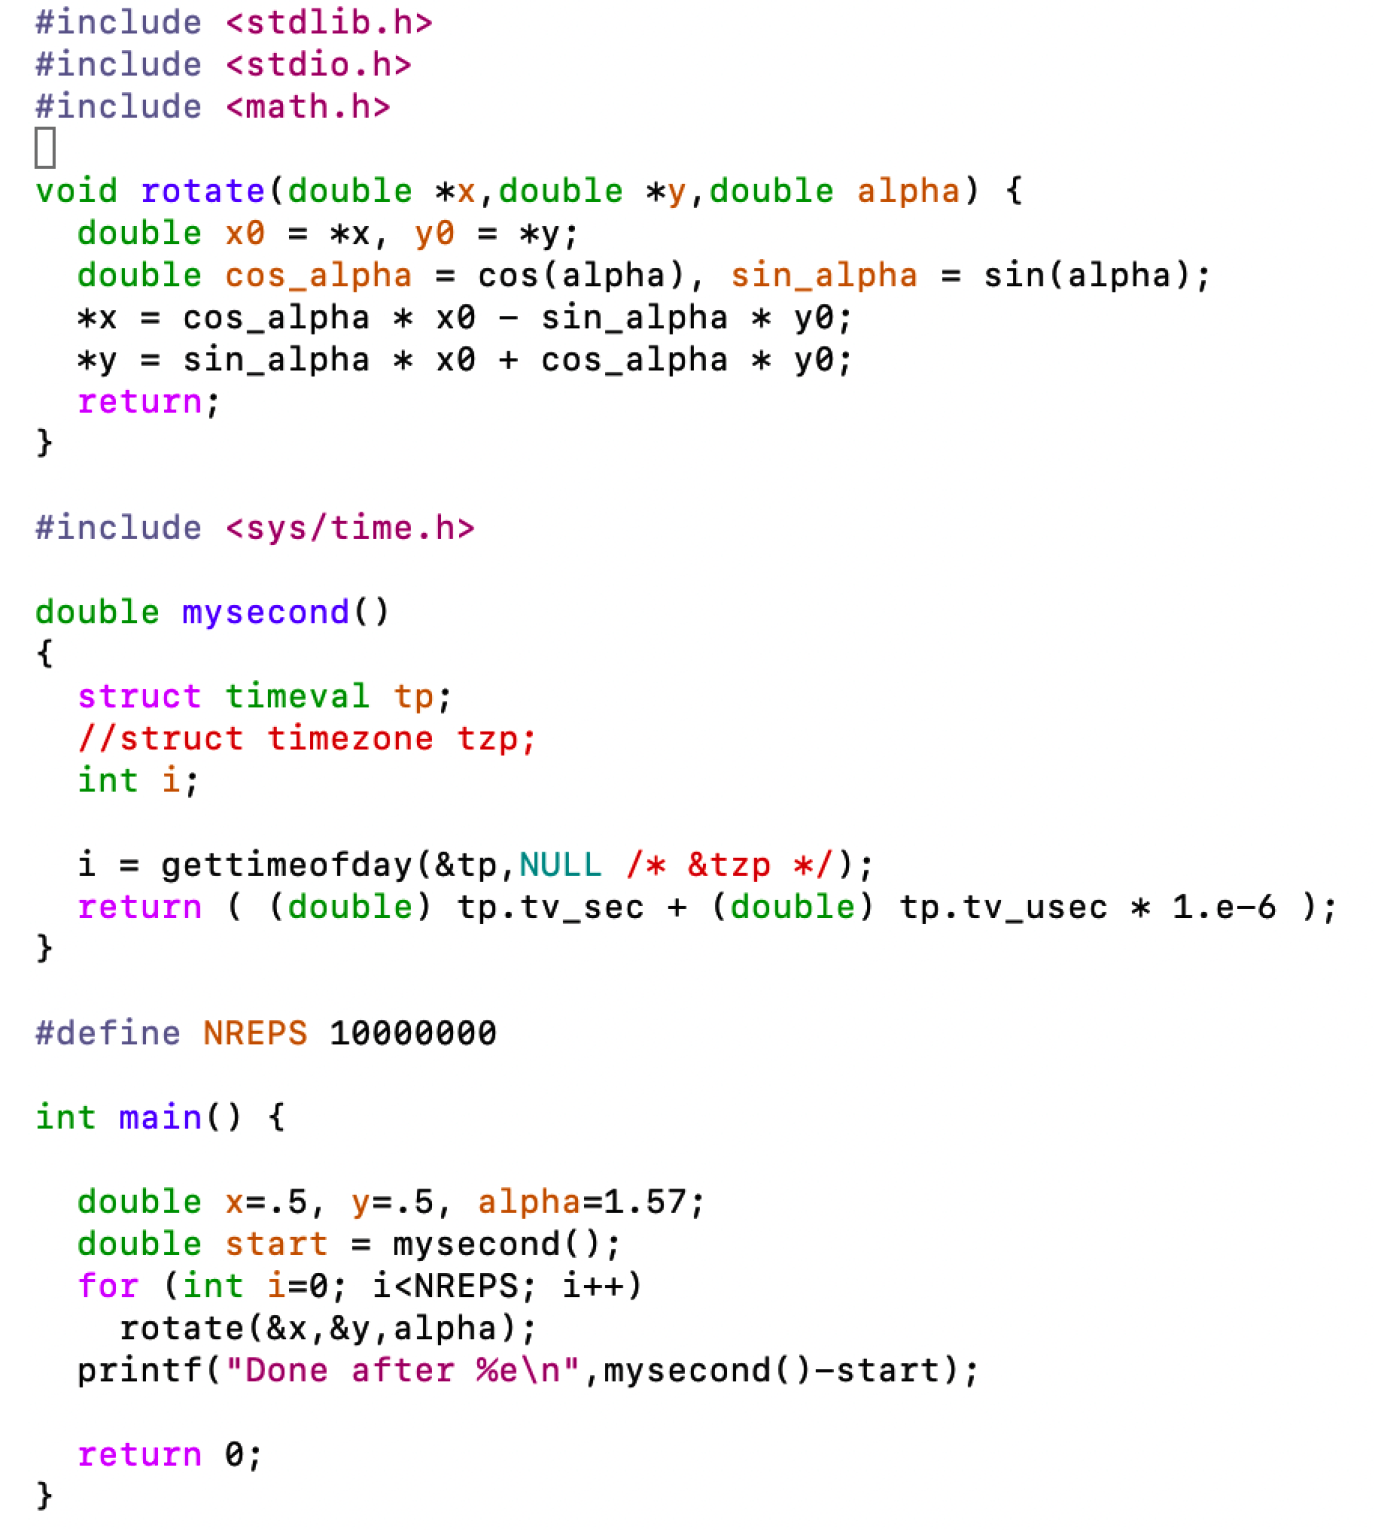
\includegraphics[scale=0.20]{graphics_hw4/rotate_c_third_iteration.png}
    \caption{Screenshot of Program "rotate.c" for Third Iteration}
    \label{fig:my_label}
\end{figure}
\pagebreak

%% Insertion of screenshot of compiler runtimes for third iteration of program

\begin{figure}[!h]
    \centering
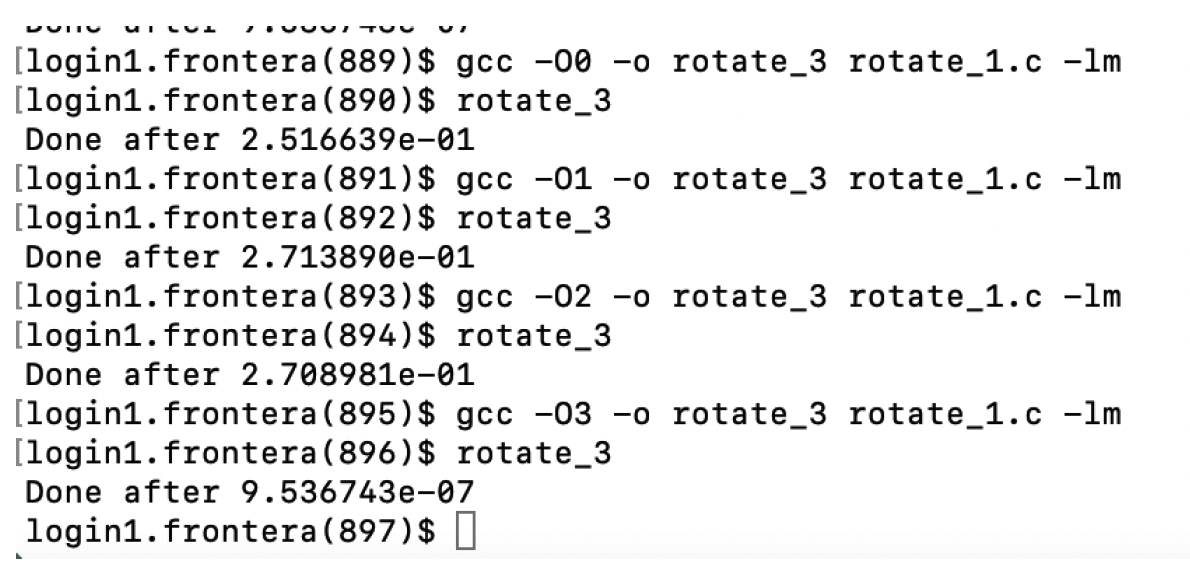
\includegraphics[scale=0.20]{graphics_hw4/compilation_runtimes_third_iteration.png}
    \caption{Screenshot of Compiler Runtimes for Third Iteration}
    \label{fig:my_label}
\end{figure}
\pagebreak

%% Summarize observations of runtimes for each of the "gcc" compilers for the third program iteration

Observations:
\begin{enumerate}
    \label{sec:math}
    \item The screenshot presented above provides the compilation commands and associated runtimes for the program, "rotate.c" in decreasing order of runtime (increasing efficiency) after the aforementioned changes to the variable declarations were applied. 
    \item As shown in the screenshot above, the transformation marginally increases the runtime of the code. 
    \item It should be noted again that the performance improvement of the runtime for each of the compilers is roughly the same as that for the runtimes in the first and second iterations of the program. 
    
\end{enumerate}
\pagebreak

%% Use "\section" command to create a new section to summarize results for second iteration of exercise:

\section{Fourth Iteration of Compile Exercise: Implementation of Macro Define Directive Statements}

In this section, images of the source file, "rotate.c" with its third set of transformations, and the compiler runtimes of the program as they appear in the terminal using compilers, "gcc - O0", "gcc -01", "gcc -02", and "gcc -03" will be provided. In this set of transformations, the variable declarations for "$cos\_alpha$" and "$sin\_alpha$" in the "rotate()" function were replaced with macro "#define" directive statements. The results from these transformations will be used to compare the runtime efficiencies of the third and fourth iterations of the program.

Provided below is a screenshot of the program, "rotate.c" in the fourth iteration (with its third set of transformations):

%% Insertion of program screenshot for fourth iteration using "\includegraphics" command

\begin{figure}[ht]
    \centering
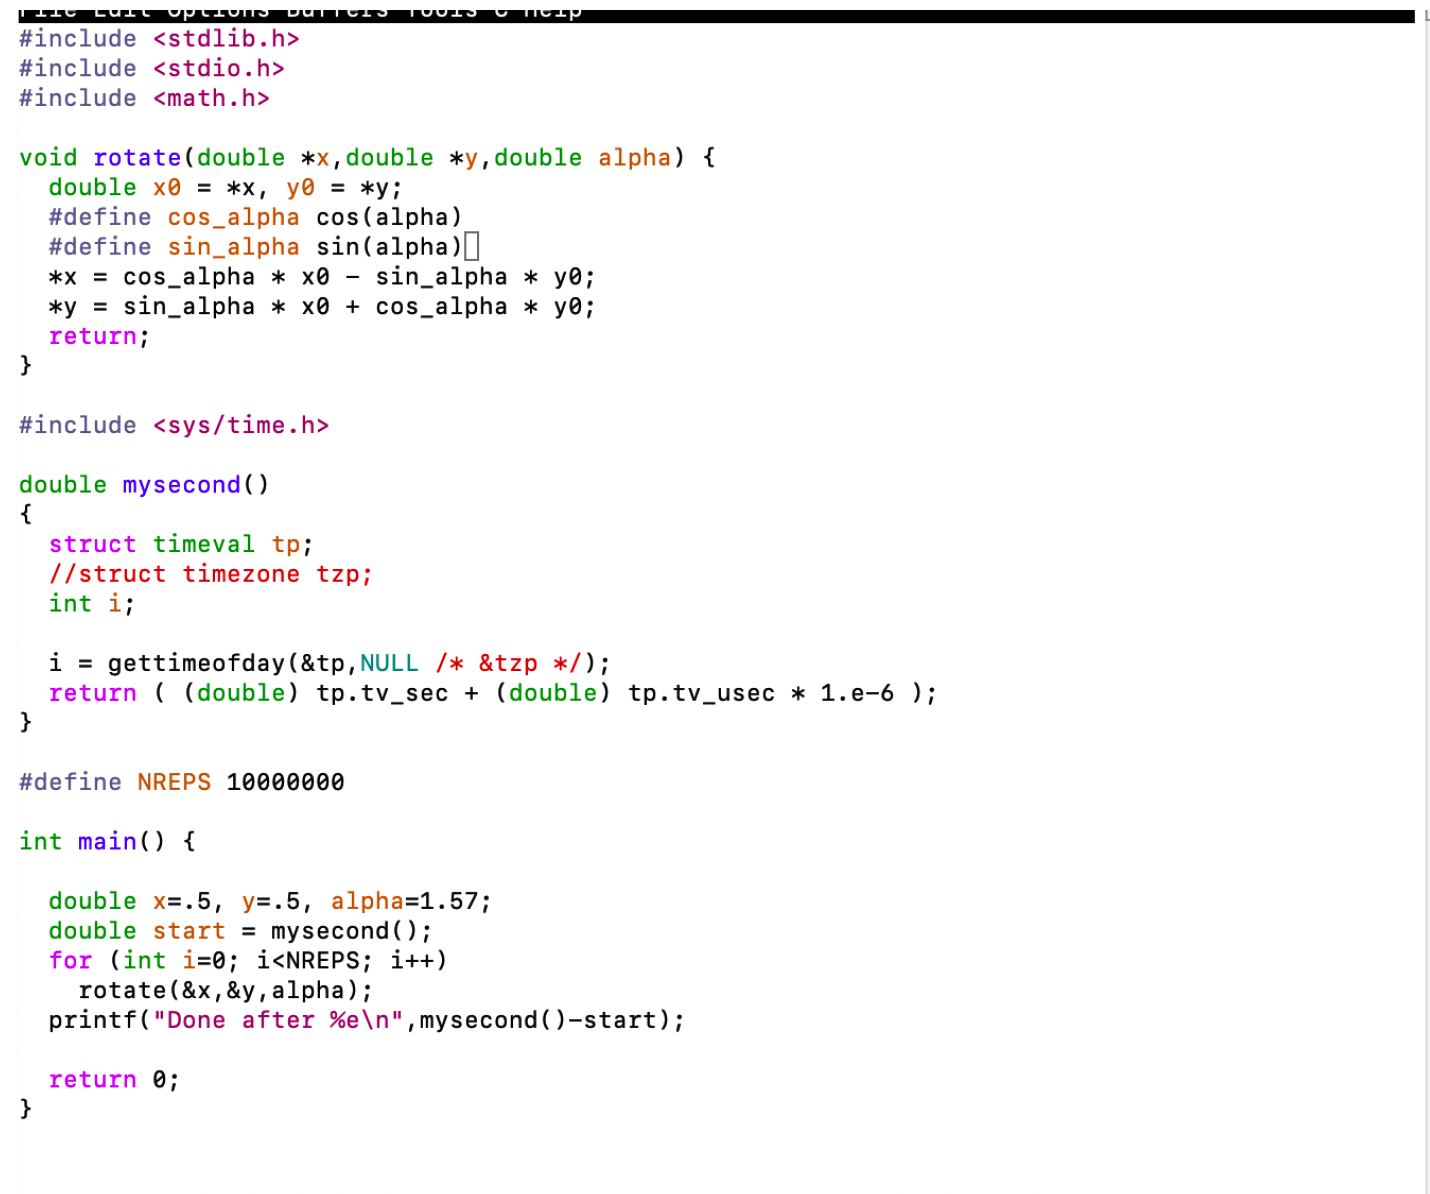
\includegraphics[scale=0.20]{graphics_hw4/rotate_c_fourth_iteration.png}
    \caption{Screenshot of Program "rotate.c" for Fourth Iteration}
    \label{fig:my_label}
\end{figure}
\pagebreak

%% Insertion of screenshot of compiler runtimes for fourth iteration of program

\begin{figure}[!h]
    \centering
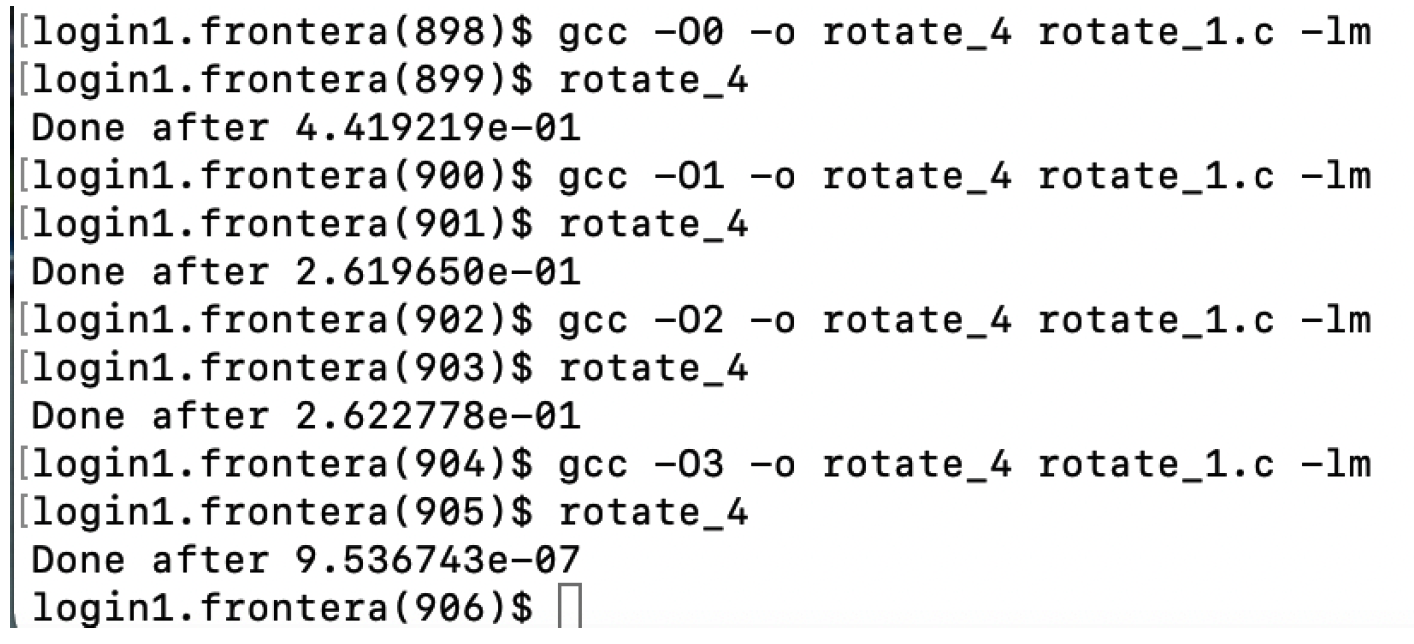
\includegraphics[scale=0.20]{graphics_hw4/compilation_runtimes_fourth_iteration.png}
    \caption{Screenshot of Compiler Runtimes for Fourth Iteration}
    \label{fig:my_label}
\end{figure}
\pagebreak

%% Summarize observations of runtimes for each of the "gcc" compilers for the fourth program iteration

Observations:
\begin{enumerate}
    \label{sec:math}
    \item The screenshot presented above provides the compilation commands and associated runtimes for the program, "rotate.c" in decreasing order of runtime (increasing effiency) after the aforementioned changes to the variable declarations of "$cos\_alpha$" and "$sin\_alpha$" were applied. 
    \item Similar to the previous transformations,  this change marginally increases the runtime of the code when the first compiler is used, marginally decreases the runtime when the second and third compiler are used, and nearly replicates the runtime when the fourth compiler is used.
    \item Again, it should be noted that the performance improvement of the runtime for each of the compilers is roughly the same as that for the runtime in the first and second iterations of the code. 
  
\end{enumerate}

\end{document}